\documentclass[12pt,twoside, a4paper, twocolumn]{article}
\usepackage[utf8]{inputenc}
\usepackage[brazil]{babel}
\usepackage[margin = 0.5in]{geometry}
\usepackage{amsmath}
\usepackage{amsthm}
\usepackage{amssymb}
\usepackage{amsthm}
\usepackage{setspace}
\usepackage[americanvoltages,fulldiodes,siunitx]{circuitikz}
\usepackage{lipsum}
\usepackage{pgfplots}
\usepackage{ifthen}
\usepackage{adjustbox}
\usepackage[section]{placeins}
\usepackage{hyperref}
\usepackage{graphicx}
\usepackage{adjustbox}
\pgfplotsset{compat=newest}
\graphicspath{ {./images/} }
%  #1 color - optional #2 x_0 #3 y_0 #4 x_f #5 y_f #6 name - optional  #7 true if adding lines to axis
\newcommand{\drawvector} [9] [color=cyan] {
\draw[line width=1.5pt,#1,-stealth](axis cs: #2, #3)--(axis cs: #4, #5) node[anchor=south west]{$#6$};
\ifthenelse{\equal{#7}{true}}{
\draw[line width=1pt,#1, dashed](axis cs: #4, #5)--(axis cs: #4, 0) node[anchor= north west]{$#8$};
\draw[line width=1pt,#1, dashed](axis cs: #4, #5)--(axis cs: 0, #5) node[anchor=south east]{$#9$};
}
{}
}
\newcommand\deriv[2]{\frac{\mathrm d #1}{\mathrm d #2}}
\title{Sétimo  Relatório de Física Experimental 2}
\author{Henrique da Silva \\ hpsilva@proton.me}
\date{\today}
\pgfplotsset{width = 10cm, compat = 1.9}
\begin{document}
\maketitle
\pagenumbering{gobble}
\newpage
%pagenumbering{roman}
\tableofcontents
\newpage

\section{Introdução}

\paragraph*{Neste relatório, vamos discutir o funcionamento de um circuito $RLC$ em série, em particular suas funções como filtro passa banda.}

\paragraph*{Também discutiremos alguns circuitos retificadores com diodos.}

\paragraph*{Todos arquivos utilizados para criar este relatório, e o relatório em si estão em:  \url{https://github.com/Shapis/ufpe_ee/tree/main/4th semester/}}


\section{Filtro Passa Banda}

\subsection{Tabela de dados}

\begin{center}
  \begin{tabular}{ |c|c|c| }
    \hline
    $F (Hz)$ & $ \frac{V_0}{V_e}$     & $\phi$ (graus) \\
             &                        &                \\
    $100$    & $0.06 \pm 5 * 10^{-2}$ & $-88 \pm 5$    \\
    $200$    & $0.17 \pm 5 * 10^{-2}$ & $-84 \pm 5$    \\
    $400$    & $0.22 \pm 5 * 10^{-2}$ & $-75 \pm 5$    \\
    $600$    & $0.34 \pm 5 * 10^{-2}$ & $-70 \pm 5$    \\
    $700$    & $0.37 \pm 5 * 10^{-2}$ & $-65 \pm 5$    \\
    $1000$   & $0.47 \pm 5 * 10^{-2}$ & $-54 \pm 5$    \\
    $1500$   & $0.62 \pm 5 * 10^{-2}$ & $-34 \pm 5$    \\
    $2000$   & $0.69 \pm 5 * 10^{-2}$ & $-17 \pm 5$    \\
    $3000$   & $0.75 \pm 5 * 10^{-2}$ & $-11 \pm 5$    \\
    $4000$   & $0.81 \pm 5 * 10^{-2}$ & $-8 \pm 5$     \\
    $5000$   & $0.82 \pm 5 * 10^{-2}$ & $0 \pm 5$      \\
    $6000$   & $0.79 \pm 5 * 10^{-2}$ & $6 \pm 5$      \\
    $8000$   & $0.78 \pm 5 * 10^{-2}$ & $16 \pm 5$     \\
    $10000$  & $0.73 \pm 5 * 10^{-2}$ & $22 \pm 5$     \\
    $15000$  & $0.63 \pm 5 * 10^{-2}$ & $35 \pm 5$     \\
    $20000$  & $0.55 \pm 5 * 10^{-2}$ & $45 \pm 5$     \\
    $30000$  & $0.43 \pm 5 * 10^{-2}$ & $48 \pm 5$     \\
    $90000$  & $0.15 \pm 5 * 10^{-2}$ & $77 \pm 5$     \\
    $150000$ & $0.09 \pm 5 * 10^{-2}$ & $87 \pm 5$     \\
    $500000$ & $0.08 \pm 5 * 10^{-2}$ & $90 \pm 5$     \\
    \hline
  \end{tabular}
\end{center}

\subsection{Grafico MonoLog de $Ve/V0$ sobre $f$}

\begin{adjustbox}{scale=0.55}
  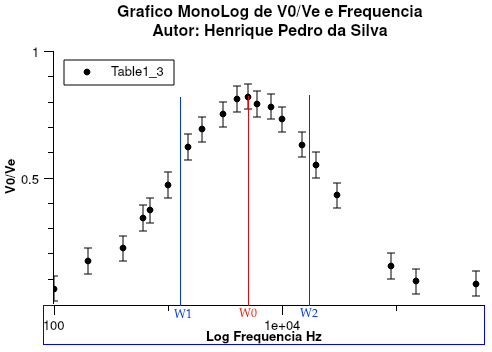
\includegraphics{Graph1.png}
\end{adjustbox}

\subsection{Diferença de fase}

\subparagraph*{A diferença de fase é aproximadamente $\pm \frac{\pi}{4}$ em $W_1$ e $W_2$}

\subsection{Figuras de Lissajous}

\paragraph{Nos casos de baixa e alta frequência a tensão $V_0$ vermelha está amplificada em 10 vezes para melhor visualização.}


\subsubsection{Baixa Frequência}

\begin{adjustbox}{scale=0.5}

  \begin{tikzpicture}
    \begin{axis}[
        ylabel={Tensao $V$},
        xlabel={Tempo $\mu s$},
        xmin = 0, xmax = 10,
        ymin = -1.2, ymax = 1.2,
        xtick distance = 2,
        ytick distance = 2,
        grid = both,
        minor tick num = 1,
        major grid style = {lightgray},
        minor grid style = {lightgray!25},
        width = 1\textwidth,
        height = 1\textwidth]
      \addplot[
        domain = 0:10,
        samples = 100,
        smooth,
        thick,
        blue,
      ] { 1.16 * cos(deg(2*pi*0.2* x))};
      \addplot[
        domain = 0:10,
        samples = 100,
        smooth,
        thick,
        red,
      ] {0.285 * sin(deg(2*pi*0.2* x))};
    \end{axis}
  \end{tikzpicture}
\end{adjustbox}


\subsubsection{Frequência de Ressonância}

\begin{adjustbox}{scale=0.5}

  \begin{tikzpicture}
    \begin{axis}[
        ylabel={Tensao $V$},
        xlabel={Tempo $10^2 \mu s$},
        xmin = 0, xmax = 10,
        ymin = -1.2, ymax = 1.2,
        xtick distance = 2,
        ytick distance = 2,
        grid = both,
        minor tick num = 1,
        major grid style = {lightgray},
        minor grid style = {lightgray!25},
        width = 1\textwidth,
        height = 1\textwidth]
      \addplot[
        domain = 0:10,
        samples = 100,
        smooth,
        thick,
        blue,
      ] { 1.16 * cos(deg(2*pi*0.2* x))};
      \addplot[
        domain = 0:10,
        samples = 100,
        smooth,
        thick,
        red,
      ] {0.822* cos(deg(2*pi*0.2* x))};
    \end{axis}
  \end{tikzpicture}
\end{adjustbox}


\subsubsection{Alta frequência}

\begin{adjustbox}{scale=0.5}

  \begin{tikzpicture}
    \begin{axis}[
        ylabel={Tensao $V$},
        xlabel={Tempo $10 ms$},
        xmin = 0, xmax = 10,
        ymin = -1.2, ymax = 1.2,
        xtick distance = 2,
        ytick distance = 2,
        grid = both,
        minor tick num = 1,
        major grid style = {lightgray},
        minor grid style = {lightgray!25},
        width = 1\textwidth,
        height = 1\textwidth]
      \addplot[
        domain = 0:10,
        samples =100,
        smooth,
        thick,
        blue,
      ] { 1.11 * sin(deg(2*pi*0.2* x))};
      \addplot[
        domain = 0:10,
        samples = 100,
        smooth,
        thick,
        red,
      ] {0.64* cos(deg(2*pi*0.2* x))};
    \end{axis}
  \end{tikzpicture}
\end{adjustbox}

\newpage

\section{Retificador de meia onda}

\subsection{Gráficos}

\subparagraph*{O que vamos observar é que a tensão medida depende da direção do diodo. }

\subparagraph*{O diodo só permite a passagem de corrente em um sentido específico. Quando a tensão da fonte inverter, o diodo bloqueia a passagem de corrente.}

\subparagraph*{Observamos este comportamento nos gráficos abaixo, um gráfico para cada sentido do diodo.}

\paragraph*{}

\begin{adjustbox}{scale=0.5}

  \begin{tikzpicture}
    \begin{axis}[
        ylabel={Tensao $V$},
        xlabel={Tempo $ms$},
        xmin = 0, xmax = 10,
        ymin = -1.2, ymax = 1.2,
        xtick distance = 2,
        ytick distance = 2,
        grid = both,
        minor tick num = 1,
        major grid style = {lightgray},
        minor grid style = {lightgray!25},
        width = 1\textwidth,
        height = 1\textwidth]
      \addplot[
        domain = 0:1,
        samples = 100,
        smooth,
        thick,
        blue,
      ] { 1 * cos(deg(2*pi*0.25* x))};
      \addplot[
        domain = 1:3,
        samples = 100,
        smooth,
        thick,
        blue,
      ] { 0};
      \addplot[
        domain = 1:3,
        samples = 100,
        smooth,
        thick,
        red,
      ] {1* cos(deg(2*pi*0.25* x))};
      \addplot[
        domain = 3:5,
        samples = 100,
        smooth,
        thick,
        blue,
      ] { 1 * cos(deg(2*pi*0.25* x))};
      \addplot[
        domain = 5:7,
        samples = 100,
        smooth,
        thick,
        blue,
      ] { 0};
      \addplot[
        domain = 5:7,
        samples = 100,
        smooth,
        thick,
        red,
      ] {1* cos(deg(2*pi*0.25* x))};
      \addplot[
        domain = 7:9,
        samples = 100,
        smooth,
        thick,
        blue,
      ] { 1 * cos(deg(2*pi*0.25* x))};
      \addplot[
        domain = 9:10,
        samples = 100,
        smooth,
        thick,
        blue,
      ] { 0};
      \addplot[
        domain = 9:10,
        samples = 100,
        smooth,
        thick,
        red,
      ] {1* cos(deg(2*pi*0.25* x))};
    \end{axis}
  \end{tikzpicture}
\end{adjustbox}

\paragraph*{}

\begin{adjustbox}{scale=0.5}

  \begin{tikzpicture}
    \begin{axis}[
        ylabel={Tensao $V$},
        xlabel={Tempo $ms$},
        xmin = 0, xmax = 10,
        ymin = -1.2, ymax = 1.2,
        xtick distance = 2,
        ytick distance = 2,
        grid = both,
        minor tick num = 1,
        major grid style = {lightgray},
        minor grid style = {lightgray!25},
        width = 1\textwidth,
        height = 1\textwidth]
      \addplot[
        domain = 0:1,
        samples = 100,
        smooth,
        thick,
        red,
      ] { 1 * cos(deg(2*pi*0.25* x))};
      \addplot[
        domain = 0:1,
        samples = 100,
        smooth,
        thick,
        blue,
      ] { 0};
      \addplot[
        domain = 1:3,
        samples = 100,
        smooth,
        thick,
        blue,
      ] {1* cos(deg(2*pi*0.25* x))};
      \addplot[
        domain = 3:5,
        samples = 100,
        smooth,
        thick,
        red,
      ] { 1 * cos(deg(2*pi*0.25* x))};
      \addplot[
        domain = 3:5,
        samples = 100,
        smooth,
        thick,
        blue,
      ] { 0};
      \addplot[
        domain = 5:7,
        samples = 100,
        smooth,
        thick,
        blue,
      ] {1* cos(deg(2*pi*0.25* x))};
      \addplot[
        domain = 7:9,
        samples = 100,
        smooth,
        thick,
        red,
      ] { 1 * cos(deg(2*pi*0.25* x))};
      \addplot[
        domain = 7:9,
        samples = 100,
        smooth,
        thick,
        blue,
      ] { 0};
      \addplot[
        domain = 9:10,
        samples = 100,
        smooth,
        thick,
        blue,
      ] {1* cos(deg(2*pi*0.25* x))};
    \end{axis}
  \end{tikzpicture}
\end{adjustbox}

\subsection{Papel do resistor}

\subparagraph*{O resistor está atuando como um controlador de corrente no circuito. }

\subsection{Processo de retificação}
\subparagraph*{Podemos observar que por meio de um circuito deste tipo podemos controlar em qual sentido o fluxo de corrente acontecerá. }

\subparagraph*{Isto nos permite filtrar uma polaridade específica da tensão de entrada.}

\newpage

\section{Retificador de onda completa}

\subsection{Efeitos do sobre a tensão antes de adicionar capacitor}

\subparagraph*{O que podemos observar é que sempre haverá uma tensão positiva no resistor, independente da polarização da fonte de entrada. }

\subparagraph*{Isto ocorre porque independente de por onde a corrente está vindo da fonte. Os diodos $D_3$ e $D_4$ a direcionam a passar de $C$ na direção de $D$.}

\subparagraph*{Isso faz com que a corrente sempre entre no resistor pelo mesmo lado.}

\subsubsection{Sistema sem capacitor}

\begin{adjustbox}{scale=0.5}

  \begin{tikzpicture}
    \begin{axis}[
        ylabel={Tensao $V$},
        xlabel={Tempo $ms$},
        xmin = 0, xmax = 10,
        ymin = -16, ymax =16,
        xtick distance = 2,
        ytick distance = 2,
        grid = both,
        minor tick num = 1,
        major grid style = {lightgray},
        minor grid style = {lightgray!25},
        width = 1\textwidth,
        height = 1\textwidth]
      \addplot[
        domain = 0:1,
        samples = 100,
        smooth,
        thick,
        red,
      ] { 16 * cos(deg(2*pi*0.25* x))};
      \addplot[
        domain = 1:3,
        samples = 100,
        smooth,
        thick,
        red,
      ] { -16 * cos(deg(2*pi*0.25* x))};
      \addplot[
        domain = 3:5,
        samples = 100,
        smooth,
        thick,
        red,
      ] {16* cos(deg(2*pi*0.25* x))};
      \addplot[
        domain = 5:7,
        samples = 100,
        smooth,
        thick,
        red,
      ] {-16* cos(deg(2*pi*0.25* x))};
      \addplot[
        domain = 7:9,
        samples = 100,
        smooth,
        thick,
        red,
      ] {16* cos(deg(2*pi*0.25* x))};
      \addplot[
        domain = 9:10,
        samples = 100,
        smooth,
        thick,
        red,
      ] {-16* cos(deg(2*pi*0.25* x))};
    \end{axis}
  \end{tikzpicture}
\end{adjustbox}


\subsection{Efeitos sobre a tensão após adicionar o capacitor}

\subparagraph*{O que vamos observar agora é que o capacitor é carregado pela fonte, e quando a tensão da entrada baixa, o capacitor entra em resposta natural e supre a tensão do resistor impedindo que a tensão deste baixe.}

\subparagraph*{E quanto mais capacitância tiver o capacitor. Menos a tensão do resistor irá diminuir quando a tensão da fonte passa pelo ponto mais baixo do seu ciclo.}

\subsubsection{Capacitor de 1 $\mu F$}

\begin{adjustbox}{scale=0.5}

  \begin{tikzpicture}
    \begin{axis}[
        ylabel={Tensao $V$},
        xlabel={Tempo $ms$},
        xmin = 0, xmax = 10,
        ymin = 10, ymax =16,
        xtick distance = 2,
        ytick distance = 2,
        grid = both,
        minor tick num = 1,
        major grid style = {lightgray},
        minor grid style = {lightgray!25},
        width = 1\textwidth,
        height = 1\textwidth]
      \addplot[
        domain = 0:1,
        samples = 100,
        smooth,
        thick,
        red,
      ] { -4*x +16};
      \addplot[
        domain = 1:2,
        samples = 100,
        smooth,
        thick,
        red,
      ] { -4 * cos(deg(2*pi*0.25* x)) + 12};
      \addplot[
        domain = 2:3,
        samples = 100,
        smooth,
        thick,
        red,
      ] { -4*(x-2) +16};
      \addplot[
        domain = 3:4,
        samples = 100,
        smooth,
        thick,
        red,
      ] { -4 * cos(deg(2*pi*0.25* (x-2))) + 12};
      \addplot[
        domain = 4:5,
        samples = 100,
        smooth,
        thick,
        red,
      ] { -4*(x-4) +16};
      \addplot[
        domain = 5:6,
        samples = 100,
        smooth,
        thick,
        red,
      ] { -4 * cos(deg(2*pi*0.25* (x-4))) + 12};
      \addplot[
        domain = 6:7,
        samples = 100,
        smooth,
        thick,
        red,
      ] { -4*(x-6) +16};
      \addplot[
        domain = 7:8,
        samples = 100,
        smooth,
        thick,
        red,
      ] { -4 * cos(deg(2*pi*0.25* (x-6))) + 12};
      \addplot[
        domain = 8:9,
        samples = 100,
        smooth,
        thick,
        red,
      ] { -4*(x-8) +16};
      \addplot[
        domain = 9:10,
        samples = 100,
        smooth,
        thick,
        red,
      ] { -4 * cos(deg(2*pi*0.25* (x-8))) + 12};
    \end{axis}
  \end{tikzpicture}
\end{adjustbox}

\subsubsection{Capacitor de 10 $\mu F$}

\begin{adjustbox}{scale=0.5}

  \begin{tikzpicture}
    \begin{axis}[
        ylabel={Tensao $V$},
        xlabel={Tempo $ms$},
        xmin = 0, xmax = 10,
        ymin = 10, ymax =16,
        xtick distance = 2,
        ytick distance = 2,
        grid = both,
        minor tick num = 1,
        major grid style = {lightgray},
        minor grid style = {lightgray!25},
        width = 1\textwidth,
        height = 1\textwidth]
      \addplot[
        domain = 0:1,
        samples = 100,
        smooth,
        thick,
        red,
      ] { -0.5*x +16};
      \addplot[
        domain = 1:2,
        samples = 100,
        smooth,
        thick,
        red,
      ] { -0.5 * cos(deg(2*pi*0.25* x)) + 15.5};
      \addplot[
        domain = 2:3,
        samples = 100,
        smooth,
        thick,
        red,
      ] { -0.5*(x-2) +16};
      \addplot[
        domain = 3:4,
        samples = 100,
        smooth,
        thick,
        red,
      ] { -0.5 * cos(deg(2*pi*0.25* (x-2))) + 15.5};
      \addplot[
        domain = 4:5,
        samples = 100,
        smooth,
        thick,
        red,
      ] { -0.5*(x-4) +16};
      \addplot[
        domain = 5:6,
        samples = 100,
        smooth,
        thick,
        red,
      ] { -0.5 * cos(deg(2*pi*0.25* (x-4))) + 15.5};
      \addplot[
        domain = 6:7,
        samples = 100,
        smooth,
        thick,
        red,
      ] { -0.5*(x-6) +16};
      \addplot[
        domain = 7:8,
        samples = 100,
        smooth,
        thick,
        red,
      ] { -0.5 * cos(deg(2*pi*0.25* (x-6))) + 15.5};
      \addplot[
        domain = 8:9,
        samples = 100,
        smooth,
        thick,
        red,
      ] { -0.5*(x-8) +16};
      \addplot[
        domain = 9:10,
        samples = 100,
        smooth,
        thick,
        red,
      ] { -0.5* cos(deg(2*pi*0.25* (x-8))) + 15.5};
    \end{axis}
  \end{tikzpicture}
\end{adjustbox}

\subsubsection{Capacitor de 100 $\mu F$}

\begin{adjustbox}{scale=0.5}

  \begin{tikzpicture}
    \begin{axis}[
        ylabel={Tensao $V$},
        xlabel={Tempo $ms$},
        xmin = 0, xmax = 10,
        ymin = 10, ymax =16,
        xtick distance = 2,
        ytick distance = 2,
        grid = both,
        minor tick num = 1,
        major grid style = {lightgray},
        minor grid style = {lightgray!25},
        width = 1\textwidth,
        height = 1\textwidth]
      \addplot[
        domain = 0:10,
        samples = 100,
        smooth,
        thick,
        red,
      ] {15.8};

    \end{axis}
  \end{tikzpicture}
\end{adjustbox}

\subsection{Processo com o capacitor}

\subparagraph*{O capacitor age como um buffer de tensão. Ele se carrega quando a tensão de entrada está alta. E se descarrega, mantendo a tensão no resistor quando a tensão de entrada passa pelo ponto baixo do seu ciclo.}

\subparagraph*{Quanto maior sua capacitancia, maior será a sua capacidade de manter a tensão do resistor. Tanto que no caso de $100 \mu F$, observamos que ele manteve a tensão do resistor completamente.}

\end{document}